Denne sektion diskuterer det proof of concept, der blev lavet til aktivitets delen af projektet, samt diskuterer hvordan data aggregeres og hvilket videre arbejde der kan være nyttig. 
Idéen ved at lave et proof of concept til fysisk aktivitet er, for at vise at det er en meget lavt hængende frugt, som nemt kan implementeres, hvorefter vi forventer den kan arbejdes videre på, på et senere tidspunkt. 
Det er dog vigtigt at selvom vi ikke bruger meget tid på denne del, understreger vi at ændringer i fysisk aktivitet er meget vigtigt, når det kommer til affektive lidelser. 

Metoden der bruges til at måle fysisk aktivitet blev valgt til at være skridt tælleren, da den tilnærmer sig fysisk aktivitet, idet at hvis man bevæger sig meget vil ens skridttæller afspejle dette, og da vi tænker at fysisk aktivitet er en meget lavt hængende frugt vil vi ikke se på andre metoder.

Eftersom skridt tælleren bruges, er det eneste, der skal gøres for at indsamle data, er at lave et sensor modul.
Sensor modulet skal derved kun bruge den indbyggede skridttæller i Android telefoner.
Derefter skal et analysemodul laves der kan udregner en aggregering af alle ens skridt for en given dato.

\subsection{Aggregering}
For at informationen samlet af skridt tælleren kan være brugbar, skal den samles på en eller anden måde.
Her vælges det at samle data for hver eneste dag, altså at alle målinger fra starten af en dag til slutningen den samme dag bliver summeret til en værdi.

\subsection{Visualisering}\label{sec:aktivitetVis}
Til at vise brugeren af systemet hvor mange skridt de har taget i løbet af en dag, er der brug for en måde at vise dette på.
Denne visualisering skal kunne bruges af brugerne til at se hvor mange skridt de har gået på en bestemt dato, men også hvordan deres antal af skridt ændre sig i løbet af en længere periode.

For at give et sådan overblik er der blevet lavet et søjlediagram, hvor hver søjle viser hvor mange skridt man har gået på en bestemt dato, et eksempel kan ses i \cref{fig:skridttaeller}.
Dette kan dog nemt komme til at se uoverskueligt ud hvis man har data for et helt år, hvilket er grunden til at zoom er blevet introduceret.
Denne funktionalitet gør at det er nemt for brugerne at få et overblik over hvordan deres antal af skridt ændres i løbet af en kort periode, men også hvordan det ændres over en længere periode.
Hvilket gør at det er nemmere for brugerne at danne et overblik over hvordan deres adfærd ændres.

\begin{figure}[h]
	\centering
	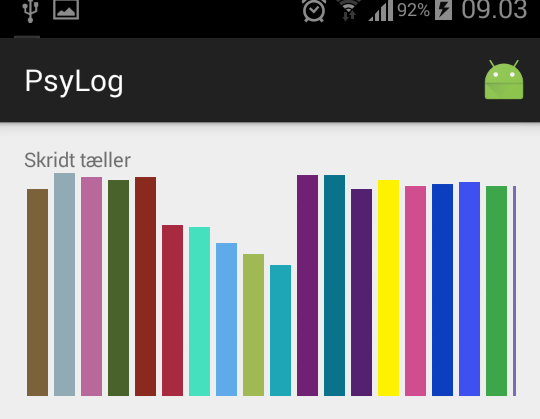
\includegraphics[scale=0.6]{visningbarchart}
	\caption{Visualisering af skridt tæller.}
	\label{fig:skridttaeller}
\end{figure}

\als{Til Ivan: Vi er usikre på om der skal skrives noget om verificering her. Det er en indbygget skridttæller fra Android vi bruger. Derudover har vi svært ved at kunne finde den absolutte sandhed for hvor fysisk aktiv man er.}